%==============================================================================
% Sjabloon poster bachproef
%==============================================================================
% Gebaseerd op document class `a0poster' door Gerlinde Kettl en Matthias Weiser
% Aangepast voor gebruik aan HOGENT door Jens Buysse en Bert Van Vreckem

\documentclass[a0,portrait]{hogent-poster}

% Info over de opleiding
\course{Bachelorproef}
\studyprogramme{toegepaste informatica}
\academicyear{2024-2025}
\institution{Hogeschool Gent, Valentin Vaerwyckweg 1, 9000 Gent}

% Info over de bachelorproef
\title{Alternatieven voor Dropbox bij Aquarius Zwemclub Lebbeke.}
\subtitle{Een onderzoek naar cloudopslag.}
\author{Luka Deserranno}
\email{Luka.Deserranno@student.hogent.be}
\supervisor{Sonia VanderMeersch}
\cosupervisor{Thomas Aelbrecht (Aquarius Zwemclub Lebbeke)}

% Indien ingevuld, wordt deze informatie toegevoegd aan het einde van de
% abstract. Zet in commentaar als je dit niet wilt.
\keywords{Cloudopslag, Angular, Node.js, Toegangsbeheer, DigitalOcean Spaces}

\begin{document}

\maketitle

\begin{abstract}
Bestandenbeheer bij kleine sportverenigingen blijft een veelvoorkomend knelpunt. Diensten zoals Dropbox en OneDrive worden vaak ingezet, maar kampen met belangrijke beperkingen: ze vereisen extra accounts, bieden beperkte controle over toegangsrechten en integreren moeilijk met bestaande digitale omgevingen.

Ook Aquarius Zwemclub Lebbeke (AZL) ondervond deze problemen. Lesgevers hadden geen uniforme toegang tot bestanden, toegangsrechten waren moeilijk beheersbaar en het beheer verliep grotendeels manueel. Dit leidde tot inefficiëntie en frustratie bij de gebruikers.

In deze bachelorproef werd onderzocht of het mogelijk is een cloudopslagoplossing te implementeren die:
\begin{itemize}
\item Naadloos integreert in het bestaande platform van AZL
\item Fijnmazige toegangscontrole per gebruiker en mapniveau mogelijk maakt
\item Beschikbaar is zonder dat lesgevers extra accounts moeten aanmaken
\item Voldoende schaalbaar en toekomstbestendig is
\end{itemize}

Als oplossing werd gekozen voor een infrastructuur gebaseerd op DigitalOcean, waarbij een eigen cloudomgeving werd opgezet met een intuïtieve gebruikersinterface, rechtstreeks toegankelijk via het interne platform van AZL. Door gebruik te maken van open-source componenten en API-koppelingen werd een oplossing gebouwd die volledig aangepast is aan de noden van de club.

Een proof of concept werd ontwikkeld en getest binnen de bestaande IT-omgeving. De resultaten tonen aan dat deze oplossing het beheer van bestanden sterk vereenvoudigt, de veiligheid verhoogt door betere toegangscontrole, en de gebruikservaring voor lesgevers aanzienlijk verbetert.

Deze aanpak biedt niet enkel voordelen voor AZL, maar kan ook dienen als model voor andere kleine sportorganisaties met gelijkaardige uitdagingen.

\end{abstract}

\begin{multicols}{2} % This is how many columns your poster will be broken into, a portrait poster is generally split into 2 columns

\section{Introductie}

Be quiet! Found them? In Mercia?! The coconut's tropical! But you are dressed as one… Well, what do you want? Knights of Ni, we are but simple travelers who seek the enchanter who lives beyond these woods.

Well, what do you want? It's only a model. Camelot! We found them. We shall say `Ni' again to you, if you do not appease us.

The nose? Shut up! Burn her! I am your king. You don't vote for kings.

You can't expect to wield supreme power just `cause some watery tart threw a sword at you! Well, we did do the nose. I don't want to talk to you no more, you empty-headed animal food trough water! I fart in your general direction! Your mother was a hamster and your father smelt of elderberries! Now leave before I am forced to taunt you a second time!

Why do you think that she is a witch? We want a shrubbery!! I don't want to talk to you no more, you empty-headed animal food trough water! I fart in your general direction! Your mother was a hamster and your father smelt of elderberries! Now leave before I am forced to taunt you a second time!

\section{Experimenten}

A newt? Camelot! Why? No, no, no! Yes, yes. A bit. But she's got a wart.

Shut up! I dunno. Must be a king. Who's that then? Look, my liege! On second thoughts, let's not go there. It is a silly place.

Shut up! Will you shut up?! No, no, no! Yes, yes. A bit. But she's got a wart. He hasn't got shit all over him. It's only a model. It's only a model.

Bring her forward! I don't want to talk to you no more, you empty-headed animal food trough water! I fart in your general direction! Your mother was a hamster and your father smelt of elderberries! Now leave 

\section{Sectie met figuur}

De {\LaTeX} figure-omgeving bepaalt zelf waar een afbeelding komt en dat is meestal niet op de plek in de tekst waar de figure-omgeving gedefinieerd wordt. Als je wilt forceren dat afbeeldingen toch in de flow van de tekst blijven, dan kan je dat zoals hieronder:

\begin{center}
  \captionsetup{type=figure}
  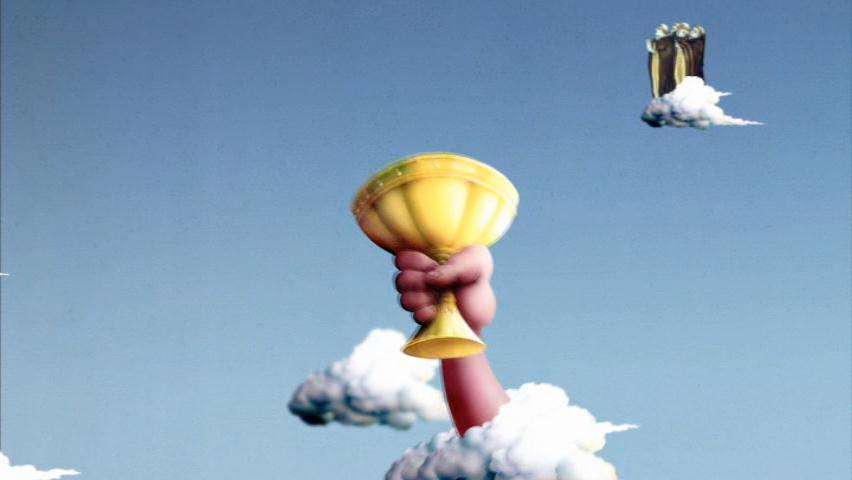
\includegraphics[width=1.0\linewidth]{grail}
  \captionof{figure}{He hasn't got shit all over him. The nose? Where'd you get the coconuts? What do you mean? We shall say `Ni' again to you, if you do not appease us}
\end{center}

Let er wel op dat dit tot problemen met bladschikking kan leiden.

\section{Conclusies}

Don't underestimate the Force. Oh God, my uncle. How am I ever gonna explain this? I suggest you try it again, Luke. This time, let go your conscious self and act on instinct. Don't be too proud of this technological terror you've constructed. The ability to destroy a planet is insignificant next to the power of the Force.

\section{Toekomstig onderzoek}

De oplossing die in deze bachelorproef werd ontwikkeld voor Aquarius Zwemclub Lebbeke, 
biedt een waardevolle blauwdruk voor andere kleine sportverenigingen die kampen met gelijkaardige uitdagingen rond documentenbeheer, 
toegangsrechten en gebruiksvriendelijkheid. Veel verenigingen beschikken over beperkte IT-kennis en infrastructuur, 
waardoor generieke oplossingen zoals Dropbox of OneDrive vaak onvoldoende afgestemd zijn op hun specifieke werking. 
Een interessante piste voor toekomstig onderzoek is het generaliseren van deze oplossing tot een flexibel en schaalbaar platform voor sportclubs. 
Dit platform zou modulaire componenten kunnen bevatten voor toegangsbeheer, cloudopslag en koppelingen met bestaande websites of ledenbeheer. 
Door gebruik te maken van S3-compatibele opslag zoals DigitalOcean Spaces, gecombineerd met een intuïtieve gebruikersinterface, 
kunnen clubs zonder technische voorkennis een veilige en geïntegreerde digitale werkomgeving opzetten. 
Verder onderzoek kan ook peilen naar automatisering van rechtenbeheer op basis van ledenrollen, gebruik van mobiele toegang, 
en optimalisatie van kostenstructuren bij grootschaliger gebruik. Zo kan het huidige proof of concept evolueren tot een breder 
inzetbare tool die bijdraagt aan digitale professionalisering binnen de sportsector.

\end{multicols}
\end{document}